\scanpage{77}
% archive foliation: 76
% Handwriting upright in the supplied scan; typescript is oppositely oriented.
\margin{\deleted{$\unsure{2}$}\quad $\mathbb Z_p($}
\margin{$\mathbb Q(i)^{\unsure{*}}$\qquad $T$}
\margin{$\unsure{B_C^0(\mathbb Z)|\operatorname{Br}_C(\mathbb Z)}$}
\figure{
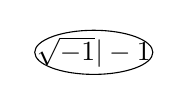
\begin{tikzpicture}
\draw (0,0) ellipse (0.75 and 0.28);
\node at (0,0) {$\unsure{\sqrt{-1}|-1}$};
\end{tikzpicture}
}
\margin{$-1$ (carré mod $p$)\qquad $p\equiv\uline{1}\quad(4)$}
\margin{$p$\qquad $p$}
\margin{$\left[\frac{-1}{p}\right]=-1$}
\margin{$\operatorname{TORS}($}

% Typescript, read in its own upright orientation.
\begin{center}
- 17 -
\end{center}

$|z_i|\leq r_i$ ; soit $M$ la borne supérieure des normes des termes de la série
pour $|z_i|=r_i$ $(1\leq i\leq p)$ ; on a donc
\[
\|\unsure{\mathbf c|C}_{n_1n_2\ldots n_p}\|\leq M/r_1^{n_1}\ldots r_p^{n_p}
\]
ce qui montre que la série entière
$(M(\frac{x_1}{r_1})^{n_1}\ldots(\frac{x_p}{r_p})^{n_p})$
est une majorante de la série donnée ; on observera que la somme de cette majorante
est $M/(1-\frac{x_1}{r_1})(1-\frac{x_2}{r_2})\ldots(1-\frac{x_p}{r_p})$
pour $|x_i|<r_i$ $(1\leq i\leq p)$.
Une autre majorante est la série obtenue par substitution de
$\sum_{i=1}^p\frac{x_i}{r_i}$ à $u$ dans la série géométrique $(Mu^n)$ ;
en effet, il est immédiat que le coefficient de $x_1^{n_1}\ldots x_p^{n_p}$
dans cette série est le produit d'un entier $\geq1$ et de
$M/r_1^{n_1}\ldots r_p^{n_p}$ ; cette nouvelle majorante a pour somme
$M/(1-\sum_{i=1}^p\frac{x_i}{r_i})$ dans un voisinage assez petit de l'origine.

\uline{2. Résolution des équations analytiques}.

THEOREME 1 .- \uline{Soient}
$f_i(x_1,\ldots,x_p\,;\,y_1,y_2,\ldots,y_p)$ $(1\leq i\leq q)$
$q$ \uline{fonctions holomorphes scalaires définies dans une partie ouverte}
$A$ \uline{de} $K^{p+q}$.

\uline{Soit} $(a_1,\ldots,a_p\,;\,b_1,\ldots,b_q)$ \uline{un point de}
$A$ \uline{tel que}
$f_i(a_1,\ldots,a_p\,;\,b_1,\ldots,b_q)=0$ \uline{pour} $1\leq i\leq q$,
\uline{et que le déterminant fonctionnel}
$\Delta=\det(\partial f_i/\partial y_j)$ \uline{soit}
$\neq0$ \uline{en ce point}.
\uline{Alors il existe un voisinage} $V$ \uline{de} $(a_1,\ldots,a_p)$
\uline{dans} $K^p$ \uline{et un système de} $q$ \uline{fonctions scalaires}
$u_i(x_1,\ldots,x_p)$ $(1\leq i\leq q)$
\uline{holomorphes dans} $V$, \uline{satisfaisant aux conditions}
$u_i(a_1,\ldots,a_p)=b_i$ $(1\leq i\leq q)$ \uline{et}
\[
(1)\qquad
f_i(x_1,\ldots,x_p\,;\,u_1(x_1,\ldots,x_p),\ldots,u_q(x_1,\ldots,x_p))=0
\quad(1\leq i\leq q)
\]
\uline{en tout point de} $V$.
\uline{En outre}, \uline{si} $v_i$ $(1\leq i\leq q)$ \uline{est un système de}
$q$ \uline{fonctions continues au point} $(a_1,\ldots,a_p)$,
\uline{définies dans un voisinage de ce point, et satisfaisant aux conditions}
$v_i(a_1,\ldots,a_p)=b_i$ $(1\leq i\leq q)$ \uline{et}
